\documentclass{beamer}
\usetheme{Copenhagen}
\usepackage[utf8]{inputenc}
\usepackage[spanish]{babel}
\usepackage{amsmath}
\usepackage{amsfonts}
\usepackage{amssymb}
\usepackage{graphicx}
\usepackage{ragged2e}
\usepackage{xcolor}
\usepackage{listings}

\usepackage{hyperref}
\hypersetup{urlcolor=blue}
\setbeamertemplate{navigation symbols}{}
\setbeamertemplate{caption}[numbered]

\definecolor{lightgrey}{rgb}{0.9,0.9,0.9}
\definecolor{darkgreen}{rgb}{0,0.6,0}

\lstset{language=[LaTeX]TeX,
texcsstyle=*\bf\color{blue},
numbers=none,
breaklines=true,
keywordstyle=\color{darkgreen},
literate=*{\{} {{\textcolor{darkgreen}\{}}{1}%
			 {\}} {{\textcolor{darkgreen}\}}}{1}%
			 {[} {{\textcolor{darkgreen}[}}{1}%
			 {]} {{\textcolor{darkgreen}]}}{1}%
			 {\$} {{\textcolor{darkgreen}\$}}{1},
commentstyle=\color{red},
frame=none,
tabsize=2,
backgroundcolor=\color{lightgrey}
}

\title{Introducci\'on a \LaTeX}
\author{Carlos Espinosa}
\date{Septiembre,2021}

\begin{document}

\begin{frame}
  \titlepage
\end{frame}

\section{Introducci\'on}
	\subsection{¿Qu\'e es \LaTeX?}
		\begin{frame}{¿Qu\'e es \LaTeX?}
			\justifying
				Es una herramienta usada para crear documentos con una apariencia profesional. Esta b\'asado en la idea \textbf{WYSIWYM} (\textit{what you see is what you mean}). Esto significa que solo te tienes que concentrar en el contenido del documento y la computadora se ocupar\'a del formato. Por lo que a diferencia de Microsoft Word o LibreOffice Writer el usuario solo escribira texto plano y \LaTeX\ har\'a el resto.
		\end{frame}

	\subsection{¿Por qu\'e aprender \LaTeX}
		\begin{frame}{¿Por qu\'e aprender \LaTeX}
			\justifying
				\LaTeX\ es usado para crear documentos cient\'ificos, libros y otras publicaciones. Permite a los usuarios hacer de manera r\'apida algunas cosas complicadas como escribir ecuaciones matem\'aticas, crear \'indices, crear referencias y crear bibliograg\'ias de manera rápida, entre otras cosas. \par
		\end{frame}
		\begin{frame}{¿Por qu\'e aprender \LaTeX}
			\justifying
				\LaTeX\ posee una gran cantidad de \textit{paquetes} que permiten a los usuarios agregar caracter\'isticas a \LaTeX\ como: crear tablas, agregar pies de p\'agina y dibujar esquemas/diagramas, etc. Los paquetes son creados por los mismos usuarios, haciendo que \LaTeX\ se convierta en una muy buena herramienta. \par
		\end{frame}
		\begin{frame}{¿Por qu\'e aprender \LaTeX}
			\justifying
				A diferencia de los editores convencionales, \LaTeX\ separa el contenido del documento y el estilo del mismo. Eso permite poder cambiar de estilo de documento en cualquier momento sin preocuparnos por el contenido. Por otro lado, si nosotros creamos un estilo de documento podemos usarlo como estándar para diversos documentos. De esta manera podemos tener \textit{plantillas} para una gran cantidad de documentos como \textit{papers}, tareas, reportes, o CVs.
		\end{frame}
\section{Escribiendo en \LaTeX}
	\subsection{Su primer documento de \LaTeX}
        \begin{frame}[fragile]{Documento b\'asico de \LaTeX}
			\LaTeX\ maneja archivos con terminaci\'on \textbf{.tex}. Basta con crear un nuevo archivo con esta terminaci\'on y editarlo ya sea con un editor de textos o con un editor especializado.
			\begin{lstlisting}
			\documentclass{article}
			\begin{document}
			    Hola Mundo
			\end{document}
			\end{lstlisting}
			Los documentos de \LaTeX\ se compilan con el comando \textit{pdflatex}, algunos editores ya tienen el comando automatizado.
			\pause
			
			Comandos importantes:
			\begin{itemize}
			    \item \lstinline!\documentclass{}!
    			\pause
			    \item \lstinline!\begin{document}...\end{document}!
			\end{itemize}
        \end{frame}
		\begin{frame}[fragile]{Estructura de un documento en \LaTeX : Preámbulo y cuerpo}
		     Partes principales de un documento en \LaTeX:
		     \begin{itemize}
		         \item En el preámbulo se pueden incluir instrucciones para activar paquetes que agregan funciones adicionales a LaTeX, así como datos generales sobre el documento que estás escribiendo. 
		         
		         \pause
		         
		         \item En el cuerpo del documento es donde escribes todo el texto que quieras que aparezca en el documento final.
		     \end{itemize}
        \end{frame}
        \begin{frame}[fragile]{Agregando opciones}
            Para agregar opciones al documento en general, las especificamos en \lstinline!\documentclass[opciones]{article}!
			\begin{lstlisting}
			\documentclass[12pt]{article}
			\begin{document}
			    Hola Mundo
			\end{document}
			\end{lstlisting}
			\pause
			\begin{lstlisting}
			\documentclass[letterpaper]{article}
			\begin{document}
			    Hola Mundo
			\end{document}
			\end{lstlisting}
        \end{frame}
        \begin{frame}[fragile]{Agregando opciones}
            Podemos combinar las opciones:
			\begin{lstlisting}
			\documentclass[12pt, letterpaper]{article}
			\begin{document}
			    Hola Mundo
			\end{document}
			\end{lstlisting}
			Otros tipos de papel:
			\begin{itemize}
			    \item a4paper
			    \item legalpaper
			\end{itemize}
        \end{frame}
		\begin{frame}[fragile]{Estructura de un documento en \LaTeX : Clases de documentos}
			Un \emph{documentclass} es un estilo de documento predefinido que contiene el formato del documento deseado. Dependiendo del tipo de documento que se va a escribir se escoge la clase de documento.
			\scriptsize
			\begin{tabular}{|c|c|}
			\hline 
			documentclass & Descripción \\ 
			\hline 
			article & \begin{tabular}{@{}c@{}}Para artículos científicos, presentaciones, \\ reportes cortos, 
			
			documentaciones de programas, invitaciones, etc\end{tabular}
			  \\ 
			\hline 
			IEEEtran & Para artículos con el formato de la IEEE \\ 
			\hline 
			proc & Una clase para expedientes basada en la clase article \\ 
			\hline 
			report & \begin{tabular}{@{}c@{}}Para reportes largos que contienen varios capítulos, \\ libros pequeños, tesis,etc 
\end{tabular}
			 \\ 
			\hline 
			book & Para libros reales \\ 
			\hline 
			slides & Para diapositivas \\ 
			\hline 
			memoir & \begin{tabular}{@{}c@{}}Basado en la clase book, con ella se puede\\ crear cualquier tipo de documento \end{tabular}
			\\ 
			\hline 
			letter & Para escribir cartas \\ 
			\hline 
			beamer & Para escribir presentaciones \\ 
			\hline 
			\end{tabular} 
			
\end{frame}
		\begin{frame}[fragile]{Estructura de un documento en \LaTeX : Clases de documentos}
			El comando \emph{\textbackslash documentclass} puede tener varias opciones. Entre estas opciones se incluyen tamaño de letra, tamaño de papel, si será a dos columnas, etc.
			
			Ejemplos:
			
			\begin{lstlisting}
	\documentclass[10pt,twoside]{report}
			\end{lstlisting}
			
			Las opciones var\'ian de clase a clase de documento.
        \end{frame}
        \begin{frame}[fragile]{Estructura de un documento en \LaTeX : T\'itulo, autor y fecha}
        \LaTeX autom\'aticamente agregar\'a el t\'itulo, autor o fecha con la instrucci\'on \lstinline!\maketitle!
        \pause
        
            Para agregar un t\'itulo usamos:
            \begin{lstlisting}
    \title{Primer documento}
            \end{lstlisting}
            \pause
            Para agregar un autor usamos:
            \begin{lstlisting}
    \author{Alan Smithee}
            \end{lstlisting}
            \pause
            Para agregar la fecha usamos
            \begin{lstlisting}
    \date{Enero, 2017}
            \end{lstlisting}
            \pause
            Todos los comandos anteriores estar\'an en el \textbf{pre\'ambulo} del documento, mientras el comando \lstinline!\maketitle! debe de ir en el \textbf{cuerpo} del documento.
        \end{frame}
		\begin{frame}{Estructura de un documento en \LaTeX}
			Comentarios sobre \LaTeX:
			\begin{itemize}
				\item Los comandos en \LaTeX\ empiezan con una diagonal invertida:
				
				\textbf{\textbackslash comando}
				\pause
				\item Los comentarios se escriben despu\'es de un símbolo de porcentaje:
				
				\textbf{\% comentario}
				\pause
				\item Hay dos forma de poner los acentos en \LaTeX:
				\begin{enumerate}
					\item Forma internacional \textbf{coraz\textbackslash'on}
					\item Forma tradicional \textbf{corazón} (Necesita un paquete para ser usada)
				\end{enumerate}
			\end{itemize}
		
		\end{frame}
	    \begin{frame}[fragile]{Usando paquetes}
	        Los paquetes de \LaTeX\ son un conjunto de instrucciones que nos permiten agregar funciones. El primer paquete que veremos ser\'a \textbf{inputenc}
	        
	        \pause
	        
	        Para usar un paquete tenemos que usar el siguiente comando:
	        
	        \begin{lstlisting}
    \usepackage[opciones]{paquete}
	        \end{lstlisting}
	        
	        \pause
	        
	        En este caso, el comando ser\'ia:

	        \begin{lstlisting}
    \usepackage[utf8]{inputenc}
	        \end{lstlisting}

\pause
	    
	        Este paquete \textit{codificar\'a} el documento. Aunque se puede usar otros, se recomienda \emph{utf8}.
	    \end{frame}
		\begin{frame}{Paquetes principales}
		Existen gran diversidad de paquetes los cuales hacen que las posibilidades de \LaTeX{} sean muy grandes. Aunque aquí se en listan los más importantes, hay muchos más.
		\footnotesize
		\begin{tabular}{|c|c|}
		\hline 
		Paquete & Descripción \\ 
		\hline 
		amsmath,amsfonts & \begin{tabular}{@{}c@{}}Nos proporcionan aún más símbolos matemáticos \\  de los que ya vienen con LaTeX por defecto. \end{tabular}
		\\ 
		\hline 
		graphicx & Necesario para incluir gráficos. \\ 
		\hline 
		geometry & Permiten modificar el tamaño de página, márgenes, etc. \\ 
		\hline 
		xcolor & Define colores en distintos modelos de color (rgb, cmy, …) \\ 
		\hline 
		babel & \begin{tabular}{@{}c@{}c@{}c@{}}Imprescindible si  quieres escribir en español o cualquier \\ otro idioma que sea distinto de inglés. Este paquete \\traduce todos los textos  estándar \\ (“figure”,”chapter”,”section”,…) al idioma deseado. \end{tabular}
		\\ 
		\hline 
		\end{tabular} 
\end{frame}
		\begin{frame}[fragile]{Estructura de un documento en \LaTeX: Cosas para recordar}
			Un documento en \LaTeX debe de tener cierta estructura:
			\begin{lstlisting}
			\documentclass{article}
			% preambulo
			\usepackage{...}
			\title{...}
			\begin{document}
			% cuerpo del documento
			Contenido
			\end{document}
			\end{lstlisting}
        \end{frame}

		\begin{frame}[fragile]{Estructura de un documento en \LaTeX : Cuerpo del documento. Notas}
			\begin{itemize}
				\item Si dejas varios espacios en blanco entre palabras, \LaTeX\ los toma como si fueran uno solo.
				\item No es necesario dejar espacios al inicio de un párrafo para indicar una sangría, \LaTeX\ ignora estos espacios y ajusta las sangrías adecuadas de manera automática.
				\item Para separar dos párrafos simplemente deja una línea en blanco entre un párrafo y el siguiente, el simple fin de línea no hace la separación.
				\item Varias líneas en blanco juntas valen lo mismo que una sola.
			\end{itemize}
\end{frame}
		\begin{frame}[fragile]{Como trabaja \LaTeX{}?}
			Veamos como formatea \LaTeX{} el texto			
			\begin{lstlisting}[basicstyle=\footnotesize
%]
]
\documentclass{article}
\author{Carlos Espinosa}
\title{Primer Documento}
\date{\today}
\begin{document}
\maketitle
Este     es el ejemplo de un p\'arrafo,
y este
sigue
siendo el mismo p\'arrafo. \LaTeX{} har\'a que todo esto se vea bien.

Este ser\'ia el segundo p\'arrafo.
% Esto es s'olo un comentario
Y aqu\'i puedes escribir m\'as cosas.
\end{document}
			\end{lstlisting}	
\end{frame}
		\begin{frame}[fragile]{Listas}
			Para hacer una lista utilizaremos el \emph{entorno} \textbf{itemize}.
			\begin{lstlisting}[basicstyle=\footnotesize]
\documentclass{article}
\author{Carlos Espinosa}
\title{Primer Documento}
\date{\today}
\begin{document}
\maketitle
Esto es una lista
\begin{itemize}
\item Primer elemento
\item Segundo elemento
\item Tercer elemento
\end{itemize}
\end{document}
			\end{lstlisting}		
			Podemos hacer listas dentro de listas!!
\end{frame}
		\begin{frame}[fragile]{Listas numeradas}
			Para hacer una lista numerada utilizaremos el \emph{entorno} \textbf{enumerate}.
			\begin{lstlisting}[basicstyle=\footnotesize]
\documentclass{article}
\author{Carlos Espinosa}
\title{Primer Documento}
\date{\today}
\begin{document}
\maketitle
Esto es una lista numerada
\begin{enumerate}
\item Primer elemento
\item Segundo elemento
\item Tercer elemento
\end{enumerate}
\end{document}
			\end{lstlisting}		
			Igual podemos hacer listas numeradas dentro de listas numeradas
\end{frame}
	\subsection{Estilos de letras}
		\begin{frame}[fragile]{Estilos de letras}
			\begin{itemize}
				\item Para poner las letras en \textbf{negritas} se utiliza el siguiente comando:
				
				\lstinline!\textbf{ejemplo}!
				
				\item Para poner las letras en \textit{cursiva} se utiliza el siguiente comando:
				
				\lstinline!\textit{ejemplo}!
				
				\item Para poner las letras \underline{subrayadas} se utiliza el siguiente comando:
				
				\lstinline!\underline{ejemplo}!
				
				\item Para poner las letras con \emph{énfasis} se utiliza el siguiente comando:
				
				\lstinline!\emph{ejemplo}!
				
				Este último depende del contexto dentro del que se use
			\end{itemize}
\end{frame}
	\subsection{Caracteres especiales}
		\begin{frame}[fragile]{Caracteres especiales}
			Algunos caracteres se tienen que escribir de forma especial.
			
			Para obtener \# , escribe \lstinline!\#!
			
			Para obtener \$ , escribe \lstinline!\$!
			
			Para obtener \% , escribe \lstinline!\%!
			
			Para obtener \& , escribe \lstinline!\&!
			
			Para obtener \_ , escribe \lstinline!\_!
			
			Para obtener \{ o \} , escribe \lstinline!\{! o \lstinline!\}!
			
			Para obtener \~\ , escribe \lstinline!\~\!
			
			Para obtener \^\ , escribe \lstinline!\^\!
			
			Para obtener \textbackslash , escribe \lstinline!\textbackslash!
			
\end{frame}
\section{Usando paquetes}
	\subsection{Modificando el documento}
		\begin{frame}[fragile]{Paquete Geometry}
			Este paquete nos permitirá modificar la geometría (tamaño y márgenes) de nuestro documento
			\begin{lstlisting}[basicstyle=\footnotesize]
\documentclass{article}
\usepackage{geometry}
\geometry{letterpaper,top=2cm,left=2cm,right=2cm,bottom=2cm}
\author{Carlos Espinosa}
\title{Primer Documento}
\date{\today}
\begin{document}
\maketitle
% texto
\end{document}
			\end{lstlisting}			
\end{frame}
		\begin{frame}[fragile]{Paquete inputenc}
			Este paquete nos permitirá modificar la codificación del texto.
			\begin{lstlisting}[basicstyle=\footnotesize]
\documentclass{article}
\usepackage{geometry}
\usepackage[utf8]{inputenc}
\geometry{letterpaper,top=2cm,left=2cm,right=2cm,bottom=2cm}
\author{Carlos Espinosa}
\title{Primer Documento}
\date{\today}
\begin{document}
\maketitle
% texto
\end{document}
			\end{lstlisting}			
\end{frame}
		\begin{frame}[fragile]{Paquete babel}
			Este se ocupará de lidiar con las particularidades propias de nuestro idioma, como la subdivisión de sílabas, nombres en español,etc.
			\begin{lstlisting}[basicstyle=\footnotesize]
\documentclass{article}
\usepackage{geometry}
\usepackage[utf8]{inputenc}
\usepackage[spanish]{babel}
\geometry{letterpaper,top=2cm,left=2cm,right=2cm,bottom=2cm}
\author{Carlos Espinosa}
\title{Primer Documento}
\date{\today}
\begin{document}
\maketitle
% texto
\end{document}
			\end{lstlisting}			
\end{frame}
	\subsection{Agregando imágenes}
		\begin{frame}[fragile]{Paquete graphicx}
			Este paquete nos permite insertar imágenes al documento. Las im\'agenes deben de estar en la misma carpeta que el archivo \textit{.tex}. El formato de las im\'agenes debe de estar en \textit{PNG} o \textit{JPG}. \LaTeX{} admite otro tipo de im\'agenes para esto se deben de usar otras opciones.
			\begin{lstlisting}[basicstyle=\tiny]
\documentclass{article}
\usepackage{graphicx}
\author{Carlos Espinosa}
\title{Primer Documento}
\date{\today}
\begin{document}
\maketitle
El universo es inmenso y parece ser homog\'eneo, a grandes escalas, a donde sea que observemos.
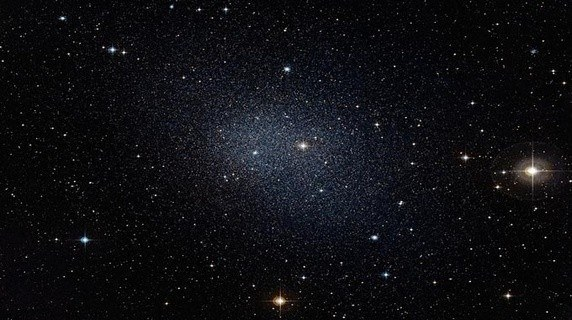
\includegraphics[scale=0.5]{universe.jpg}
Hay una imagen del universo arriba.
\end{document}
			\end{lstlisting}			
\end{frame}
		\begin{frame}[fragile]{Paquete graphicx. Cosas útiles}
			A las im\'agenes se les puede poner t\'itulo, una etiqueta y referenciarlas bajo el entorno de \textbf{figure}
			\begin{lstlisting}[basicstyle=\tiny]
\documentclass{article}
\usepackage{grpahicx}
\author{Carlos Espinosa}
\title{Primer Documento}
\date{\today}
\begin{document}
\maketitle
\begin{figure}
	\centering
	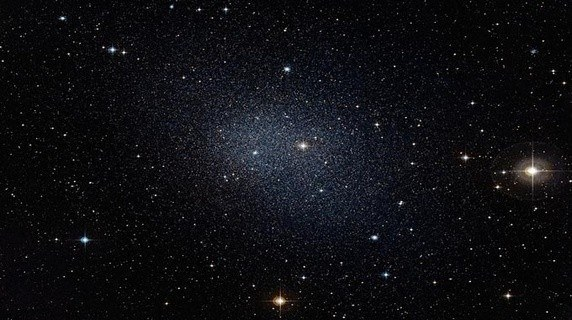
\includegraphics[scale=0.25\textwidth]{universe.jpg}
	\caption{Que bonito universo}
	\label{fig:uni}
\end{figure}
En la figura \ref{fig:uni} podemos ver una imagen de una parte del universo. En la p\'agina \pageref{fig:uni} est\'a la misma figura.
\end{document}
			\end{lstlisting}		
\end{frame}
	\subsection{Escribiendo ecuaciones}
		\begin{frame}[fragile]{Escribiendo ecuaciones}
\LaTeX por si solo contiene herramientas para escribir matem\'aticas b\'asicas. Pero si se necesitan escribir f\'ormulas m\'as complicadas se recomienda usar el paquete \textbf{amsmath} o \textbf{mathtools}. (Este segundo carga amsmath)
\begin{lstlisting}[
    basicstyle=\small, %or \small or \footnotesize etc.
]
\usepackage{amsmath}
\usepackage{amsfonts}
\end{lstlisting}
Existen dos entornos en \LaTeX: el modo \textit{inline} y el modo \textit{display}. El modo \textit{inline} escribe la expresi\'on sobre la misma l\'inea de texto. El modo \textit{display} lo hace en una secci\'on diferente		
\end{frame}
		\begin{frame}[fragile]{Modos. Inline}
			El modo inline se hace por medio de \$...\$
			\begin{lstlisting}[basicstyle=\small]
En la ecuaci\'on $\dfrac{1}{2}x^{2}+3y^{3/2}-1 = 0$ tenemos un comportamiento polinomial.
			\end{lstlisting}
			Otras formas de llamar al modo inline es con:
			\begin{itemize}
				\item \lstinline!\(...\)!
				\item \lstinline!$...$!
				\item \lstinline!\begin{math}...\end{math}!
			\end{itemize}
\end{frame}
		\begin{frame}[fragile]{Modos. Display}
			El modo display se accesa por medio de:
			\begin{itemize}
				\item $\mathbf{\rightarrow}$\lstinline!\[...\]! Sin n\'umero
				\item \lstinline!$$...$$!
				\item \lstinline!\begin{displaymath}...\end{displaymath}!
				\item $\mathbf{\rightarrow}$\lstinline!\begin{equation}...\end{equation}!
			\end{itemize}
			Los resaltados en color verde son los que se usan con m\'as frecuencia. 
\end{frame}
\section{Cosas extras de \LaTeX}
	\subsection{Nuevas l\'ineas y p\'arrafos}
		\begin{frame}[fragile]{Nuevas l\'ineas y p\'arrafos}
			Cuando uno esta escribiendo, es frecuente utilizar una nueva l\'inea. Basta con dejar en el texto, un espacio entre texto. Tambi\'en se pueden usar los comandos $\backslash$\textbf{newline} o con $\backslash \backslash$\\
Hay otro comando similar que es $\backslash$par que es an\'alogo a dejar una l\'inea en blanco entre bloques de texto.
\end{frame}
	\subsection{Secciones y subsecciones}
		\begin{frame}[fragile]{Secciones y subsecciones}
			Podemos organizar nuestro texto por secciones y sub secciones (incluso un tercer nivel subsub secciones). Tambi\'en podemos crear cap\'itulo. Los comandos para las distintas secciones son:
			\begin{itemize}
				\item \textbackslash chapter{...} (Clase de documento \emph{book})
				\item \textbackslash section{...}
				\item \textbackslash subsection{...}
				\item \textbackslash subsubsection{...}
			\end{itemize}
			Existe un comando que crear\'a de forma autom\'atica un \'indice bas\'ndose en todas las divisiones que hayamos hecho a lo largo del texto.
\end{frame}
	\subsection{Tablas}
	\begin{frame}[fragile]{Creando tablas}
	    La creaci\'on de tablas en \LaTeX\ es ``sencilla''. Para crear una tabla utilizaremos el entorno \textit{tabular}.
	    \begin{lstlisting}[basicstyle=\small]
\begin{center}
\begin{tabular}{ c c c }	    
 cell1 & cell2 & cell3 \\ 
 cell4 & cell5 & cell6 \\
 cell7 & cell8 & cell9    
\end{tabular}
\end{center}
	    \end{lstlisting}
	\end{frame}
		\begin{frame}[fragile]{A\~nadiendo bordes}
			Si queremos a\~nadir bordes el comando se transforma en:
			\begin{lstlisting}[basicstyle=\small]
\begin{center}
\begin{tabular}{ |c|c|c| } 
 \hline
 cell1 & cell2 & cell3 \\ 
 cell4 & cell5 & cell6 \\ 
 cell7 & cell8 & cell9 \\ 
 \hline
\end{tabular}
\end{center}
			\end{lstlisting}
\end{frame}

		\begin{frame}[fragile]{Títulos,referencias,etc.}
			Al igual que con las imagenes, y realmente con cualquier objeto de \LaTeX, podemos agregarle un t\'itulo y una etiqueta para referenciar una tabla:
			\begin{lstlisting}[basicstyle=\tiny]
Tabla \ref{tabla:datos} es un ejemplo de como referencias elementos de \LaTeX.
 
\begin{table}[h!]
\centering
\begin{tabular}{||c c c c||} 
 \hline
 Col1 & Col2 & Col2 & Col3 \\ 
 \hline\hline
 1 & 6 & 87837 & 787 \\ 
 2 & 7 & 78 & 5415 \\
 3 & 545 & 778 & 7507 \\
 4 & 545 & 18744 & 7560 \\
 5 & 88 & 788 & 6344 \\
 \hline
\end{tabular}
\caption{Tabla para probar t\'itulos y referencias}
\label{table:datos}
\end{table}
			\end{lstlisting}
\end{frame}

\end{document}
%%% Local Variables:
%%% mode: latex
%%% TeX-master: t
%%% End:
